\documentclass{article}
\usepackage[a4paper, total={17cm,23.7cm}]{geometry}
\usepackage[utf8]{inputenc}
\usepackage[T1]{fontenc}
\usepackage{graphicx}
\usepackage[export]{adjustbox}
\usepackage{csvsimple}

\renewcommand{\figurename}{Karte}
\renewcommand{\listfigurename}{Karten}

\begin{document}
    \section*{Entfernungen} Die Entfernungen sind ausgehend von Gabelungen und
    Einmündungen aus gerechnet -- also im Bürgerpark von der Gabelung am
    Portikus (direkt am RSV-Gelände) und dem Zusammenfluss der Okerarme nördlich
    der Innenstadt. \\
    \begin{center}
        \csvautotabular[separator=semicolon]{distances.csv}
    \end{center}
    
    \section*{Abschnittslängen}
    
    \begin{center}
        \csvautotabular[separator=semicolon]{segments.csv}
    \end{center}    
    
    \section*{Anmerkungen}
    Die Entfernungen beziehen sich auf die in OpenStreetMap vorhandenen,
    repräsentativen Linien von Wasserläufen und ggf. hinzugefügte Routen auf
    Seen. Die Entfernungen sind sowohl auf der Karte als auch in der Tabelle auf 5~m gerundet.    

    \listoffigures
    
    \begin{figure}[!h]
        \centering
        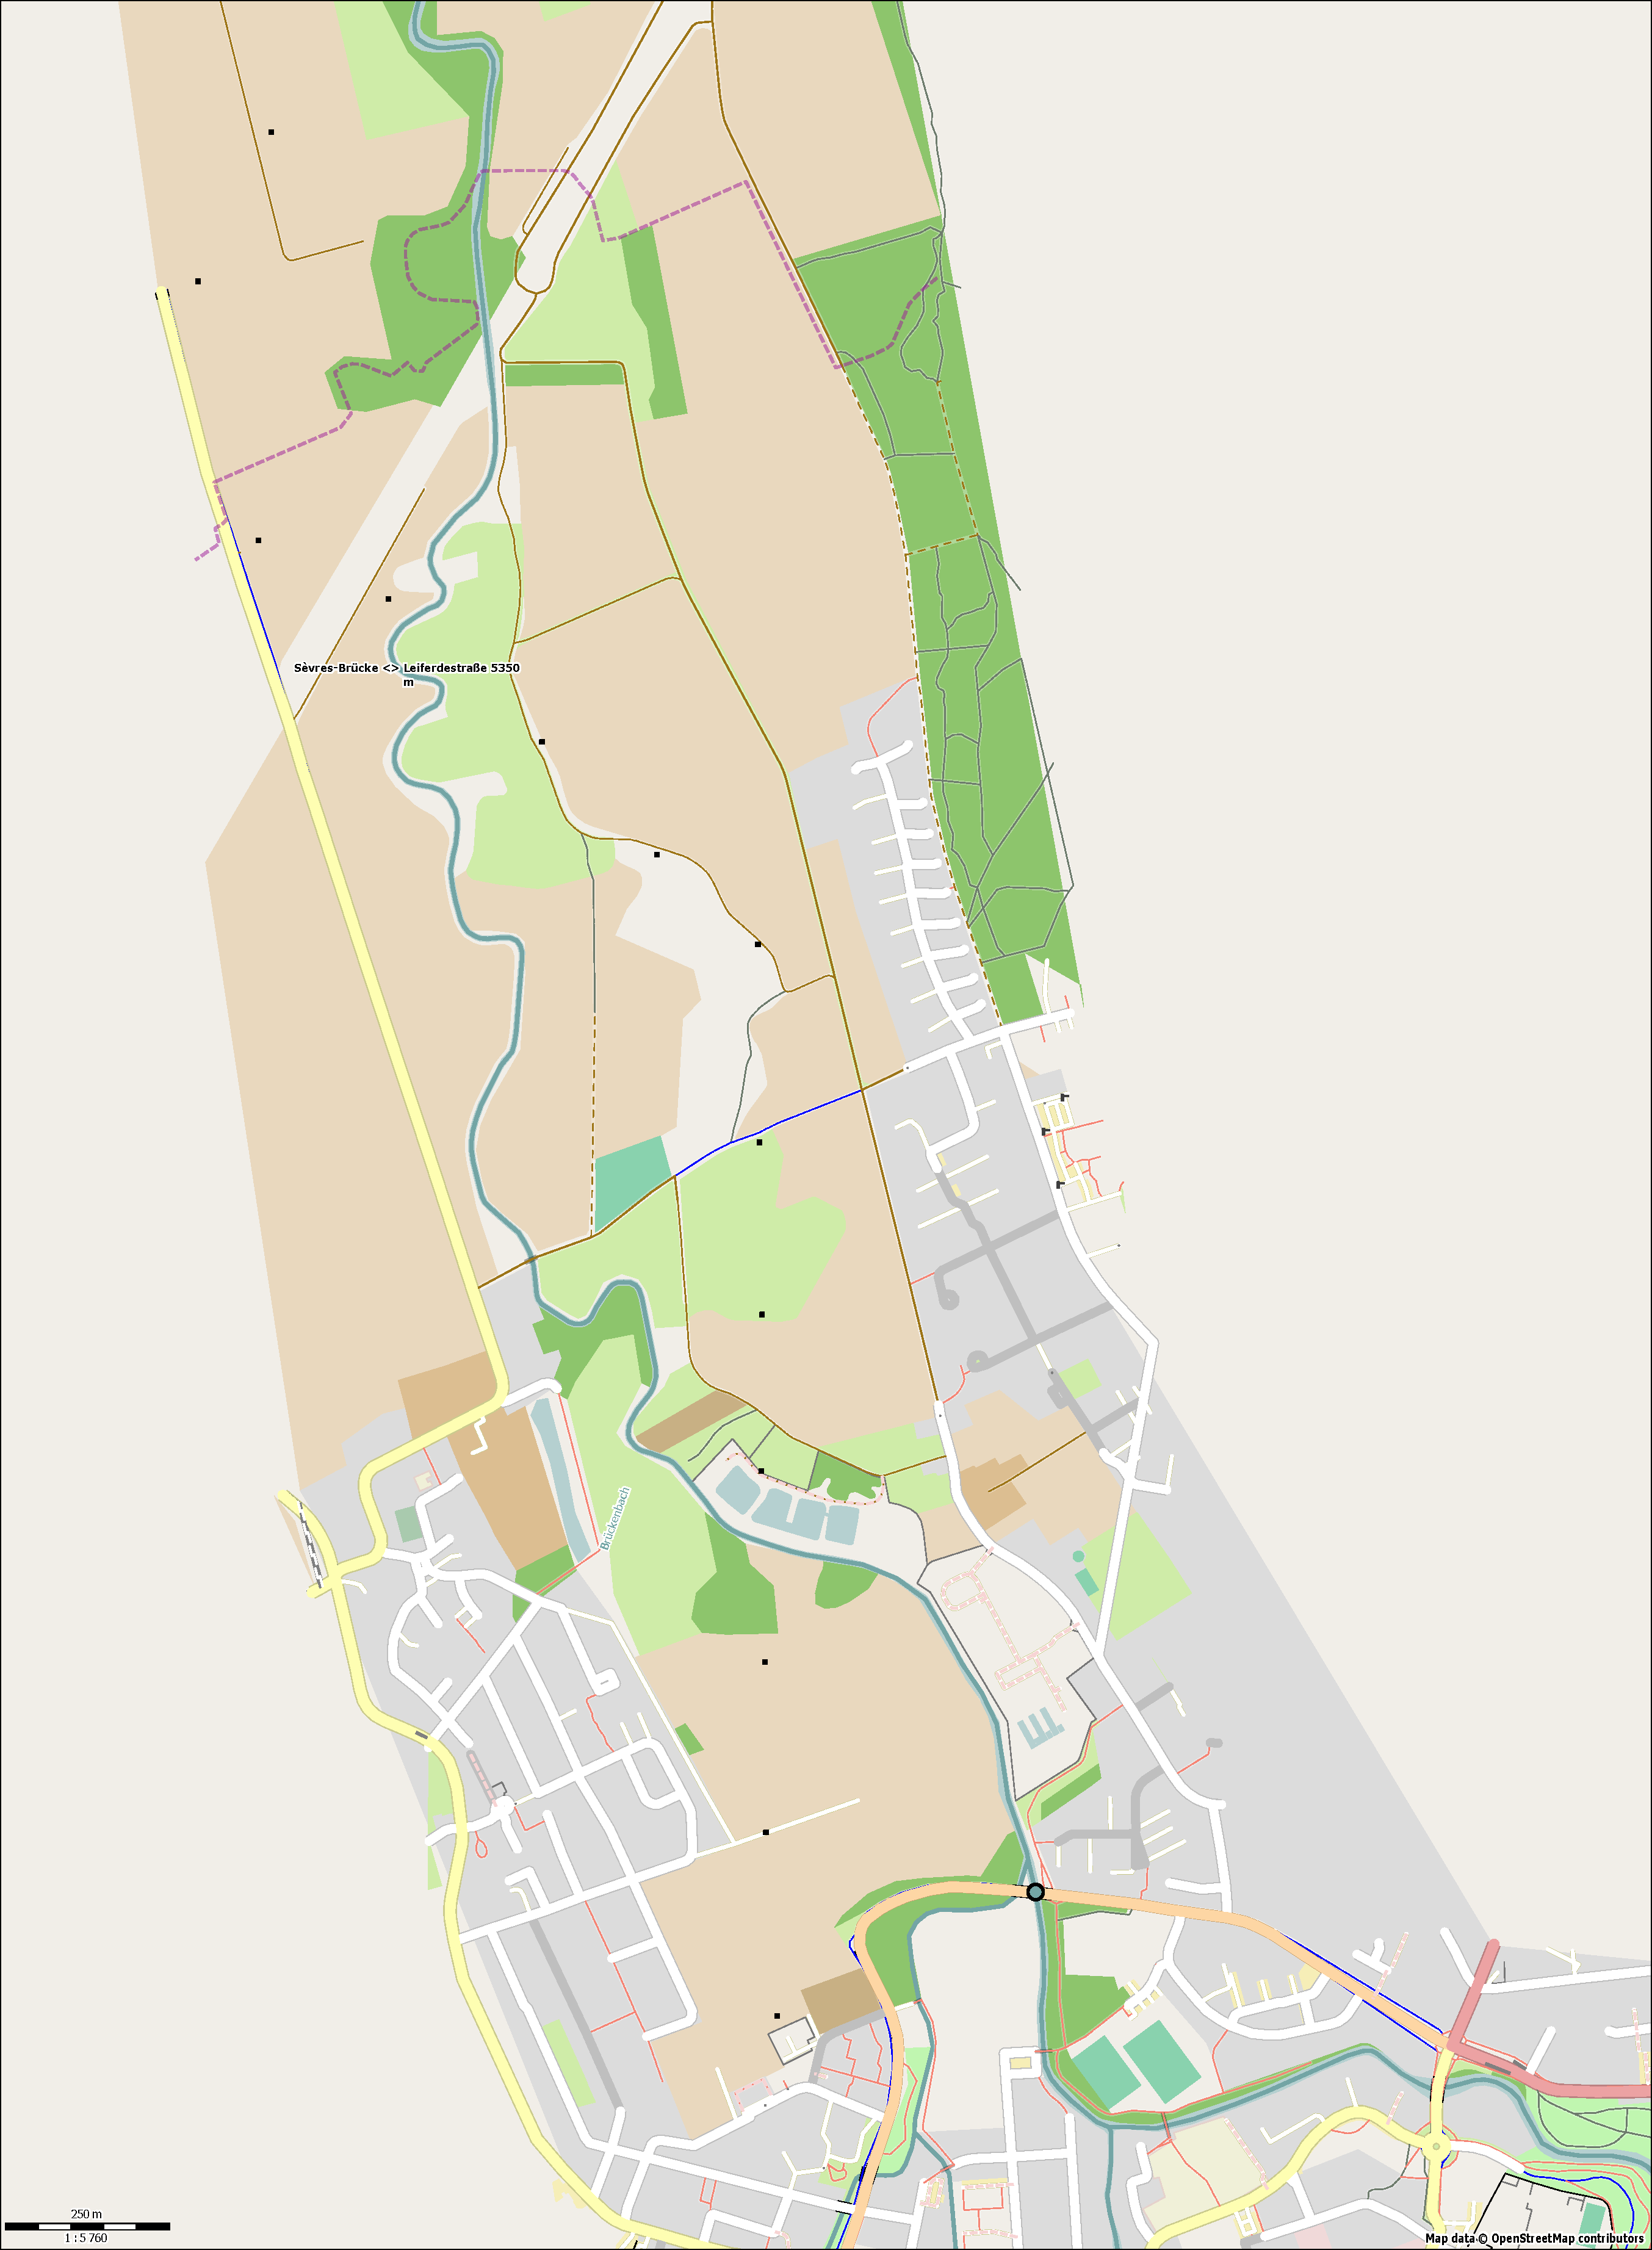
\includegraphics[max size={\textwidth}{0.95\textheight}]{../Result/WF.pdf}
        \caption{Wolfenbüttel-Nord}
        \label{fig:map_WF}
    \end{figure}
    \newpage
    
    \begin{figure}[!h]
        \centering
        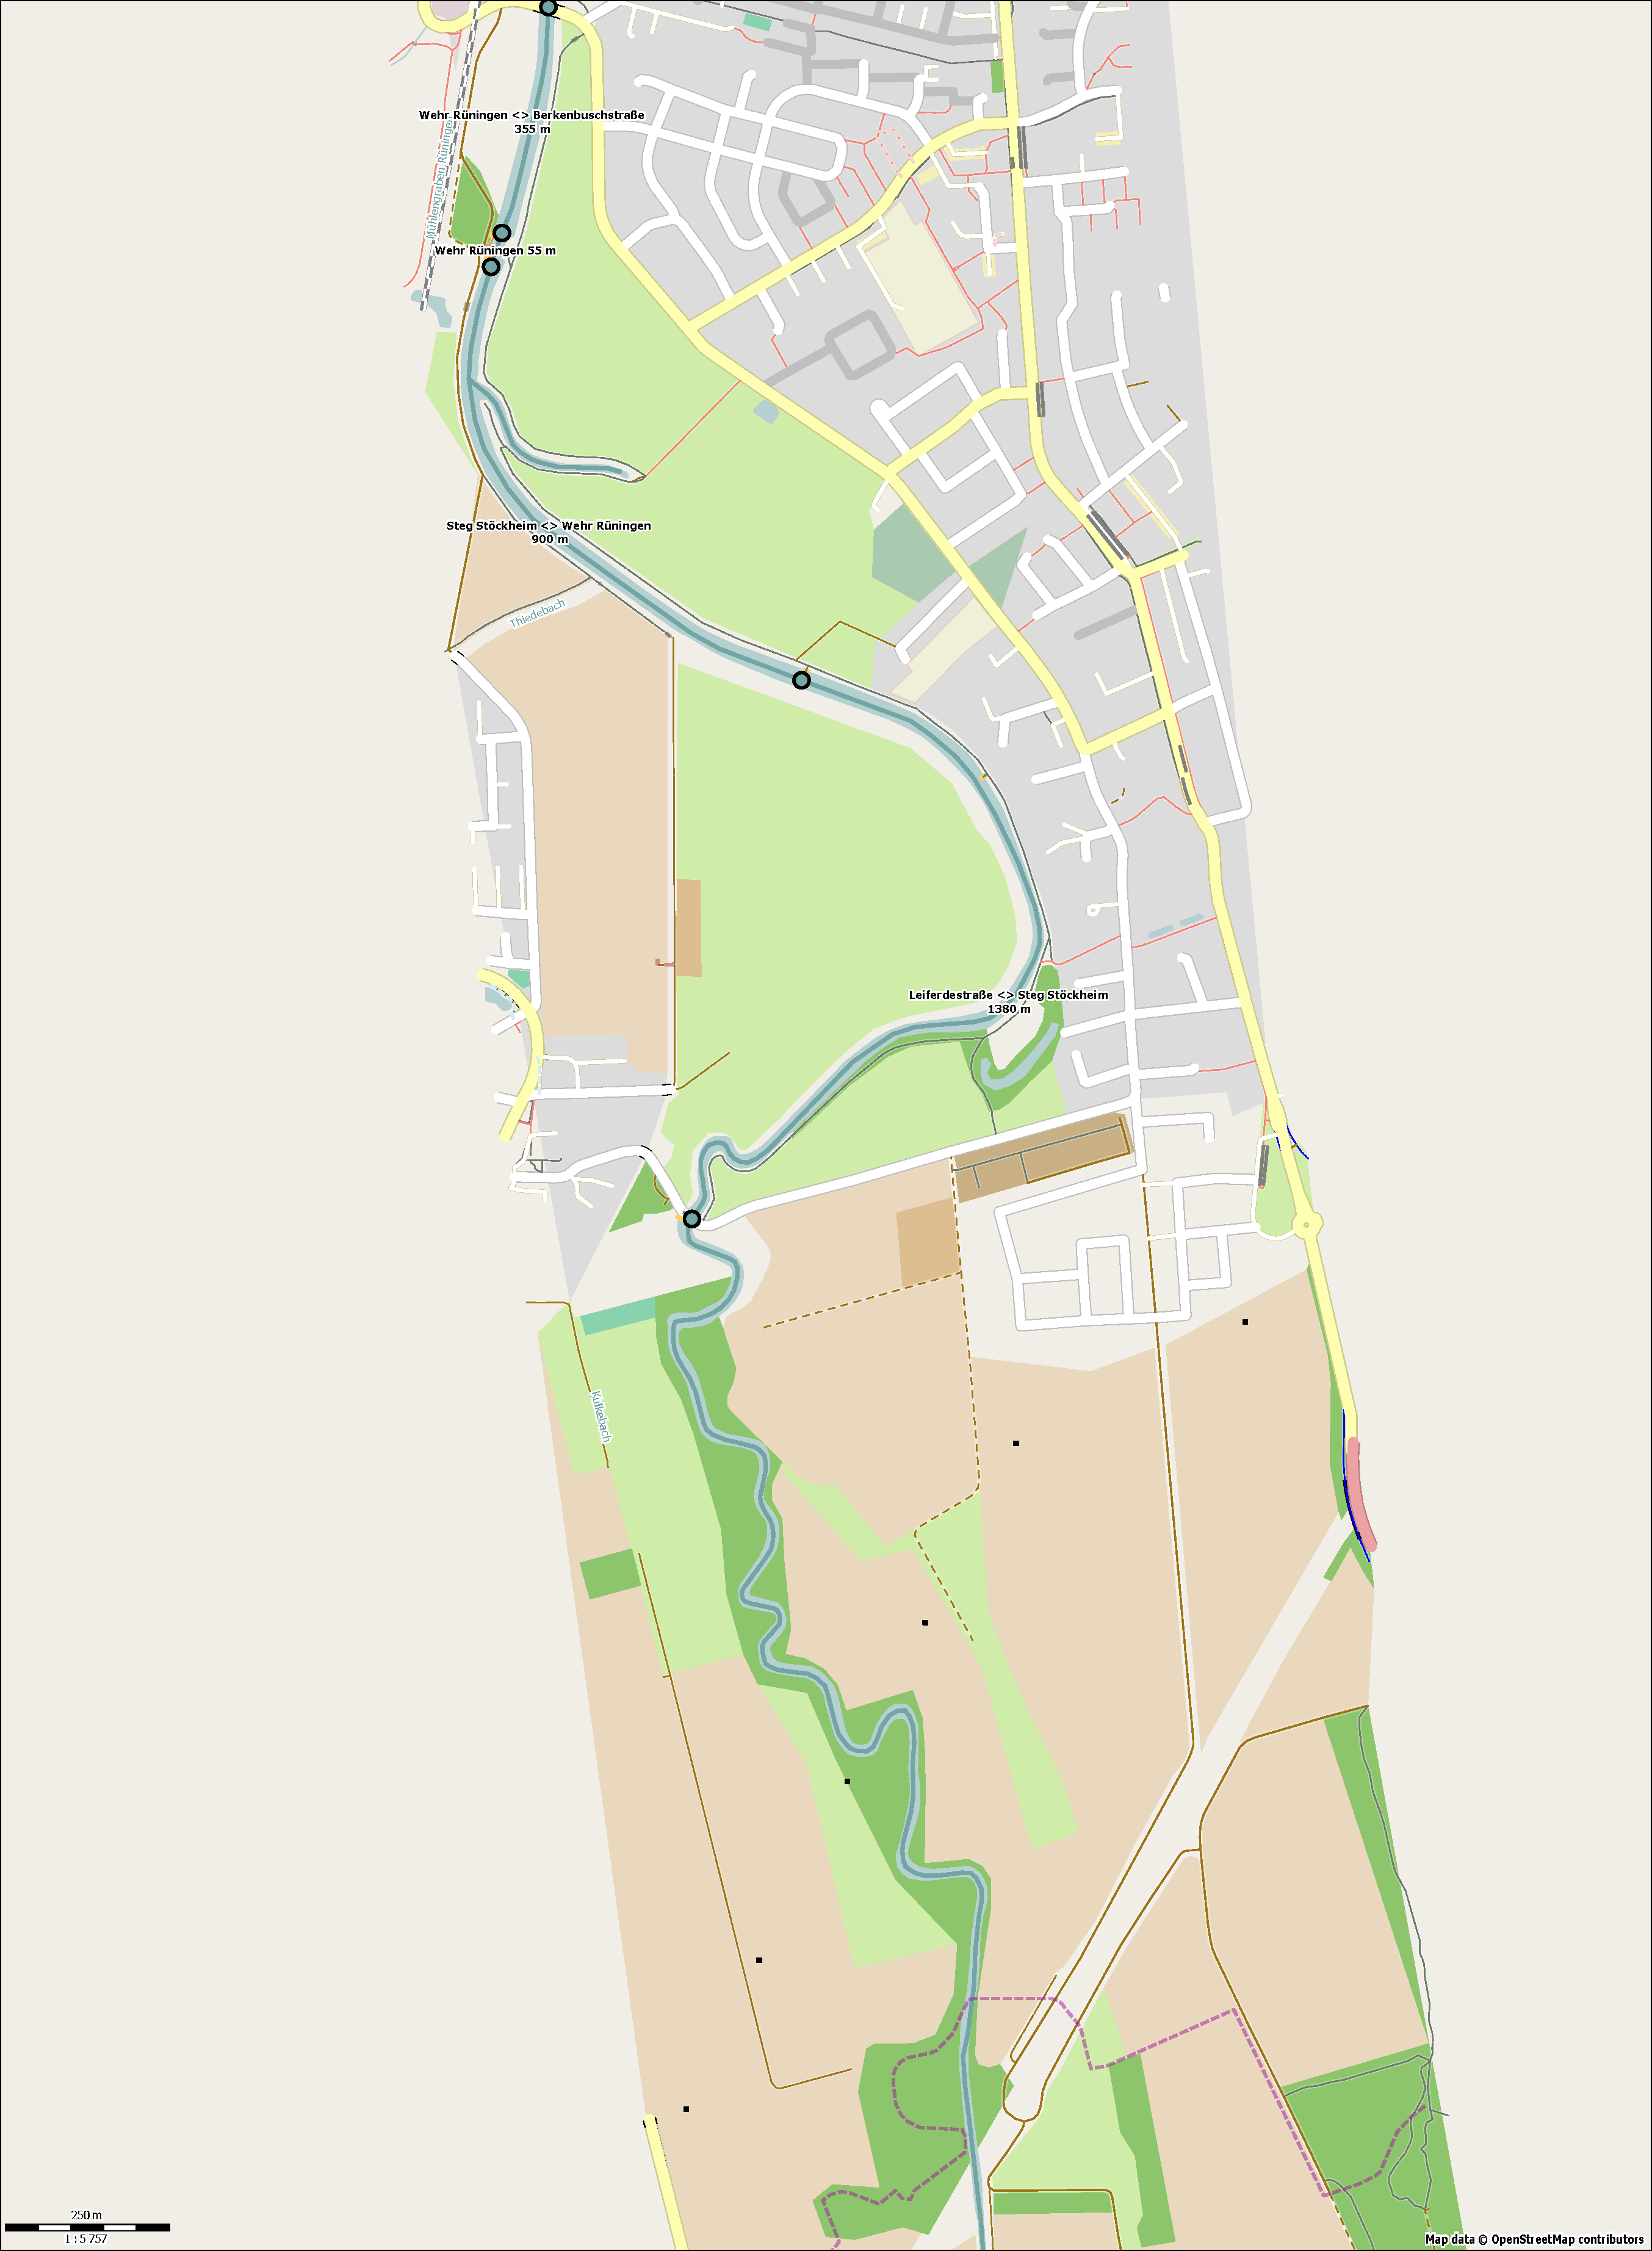
\includegraphics[max size={\textwidth}{0.95\textheight}]{../Result/BS_Sued.pdf}
        \caption{Braunschweig-Stöckheim}
        \label{fig:map_BS1}
    \end{figure}
    \newpage
    
    \begin{figure}[!h]
        \centering
        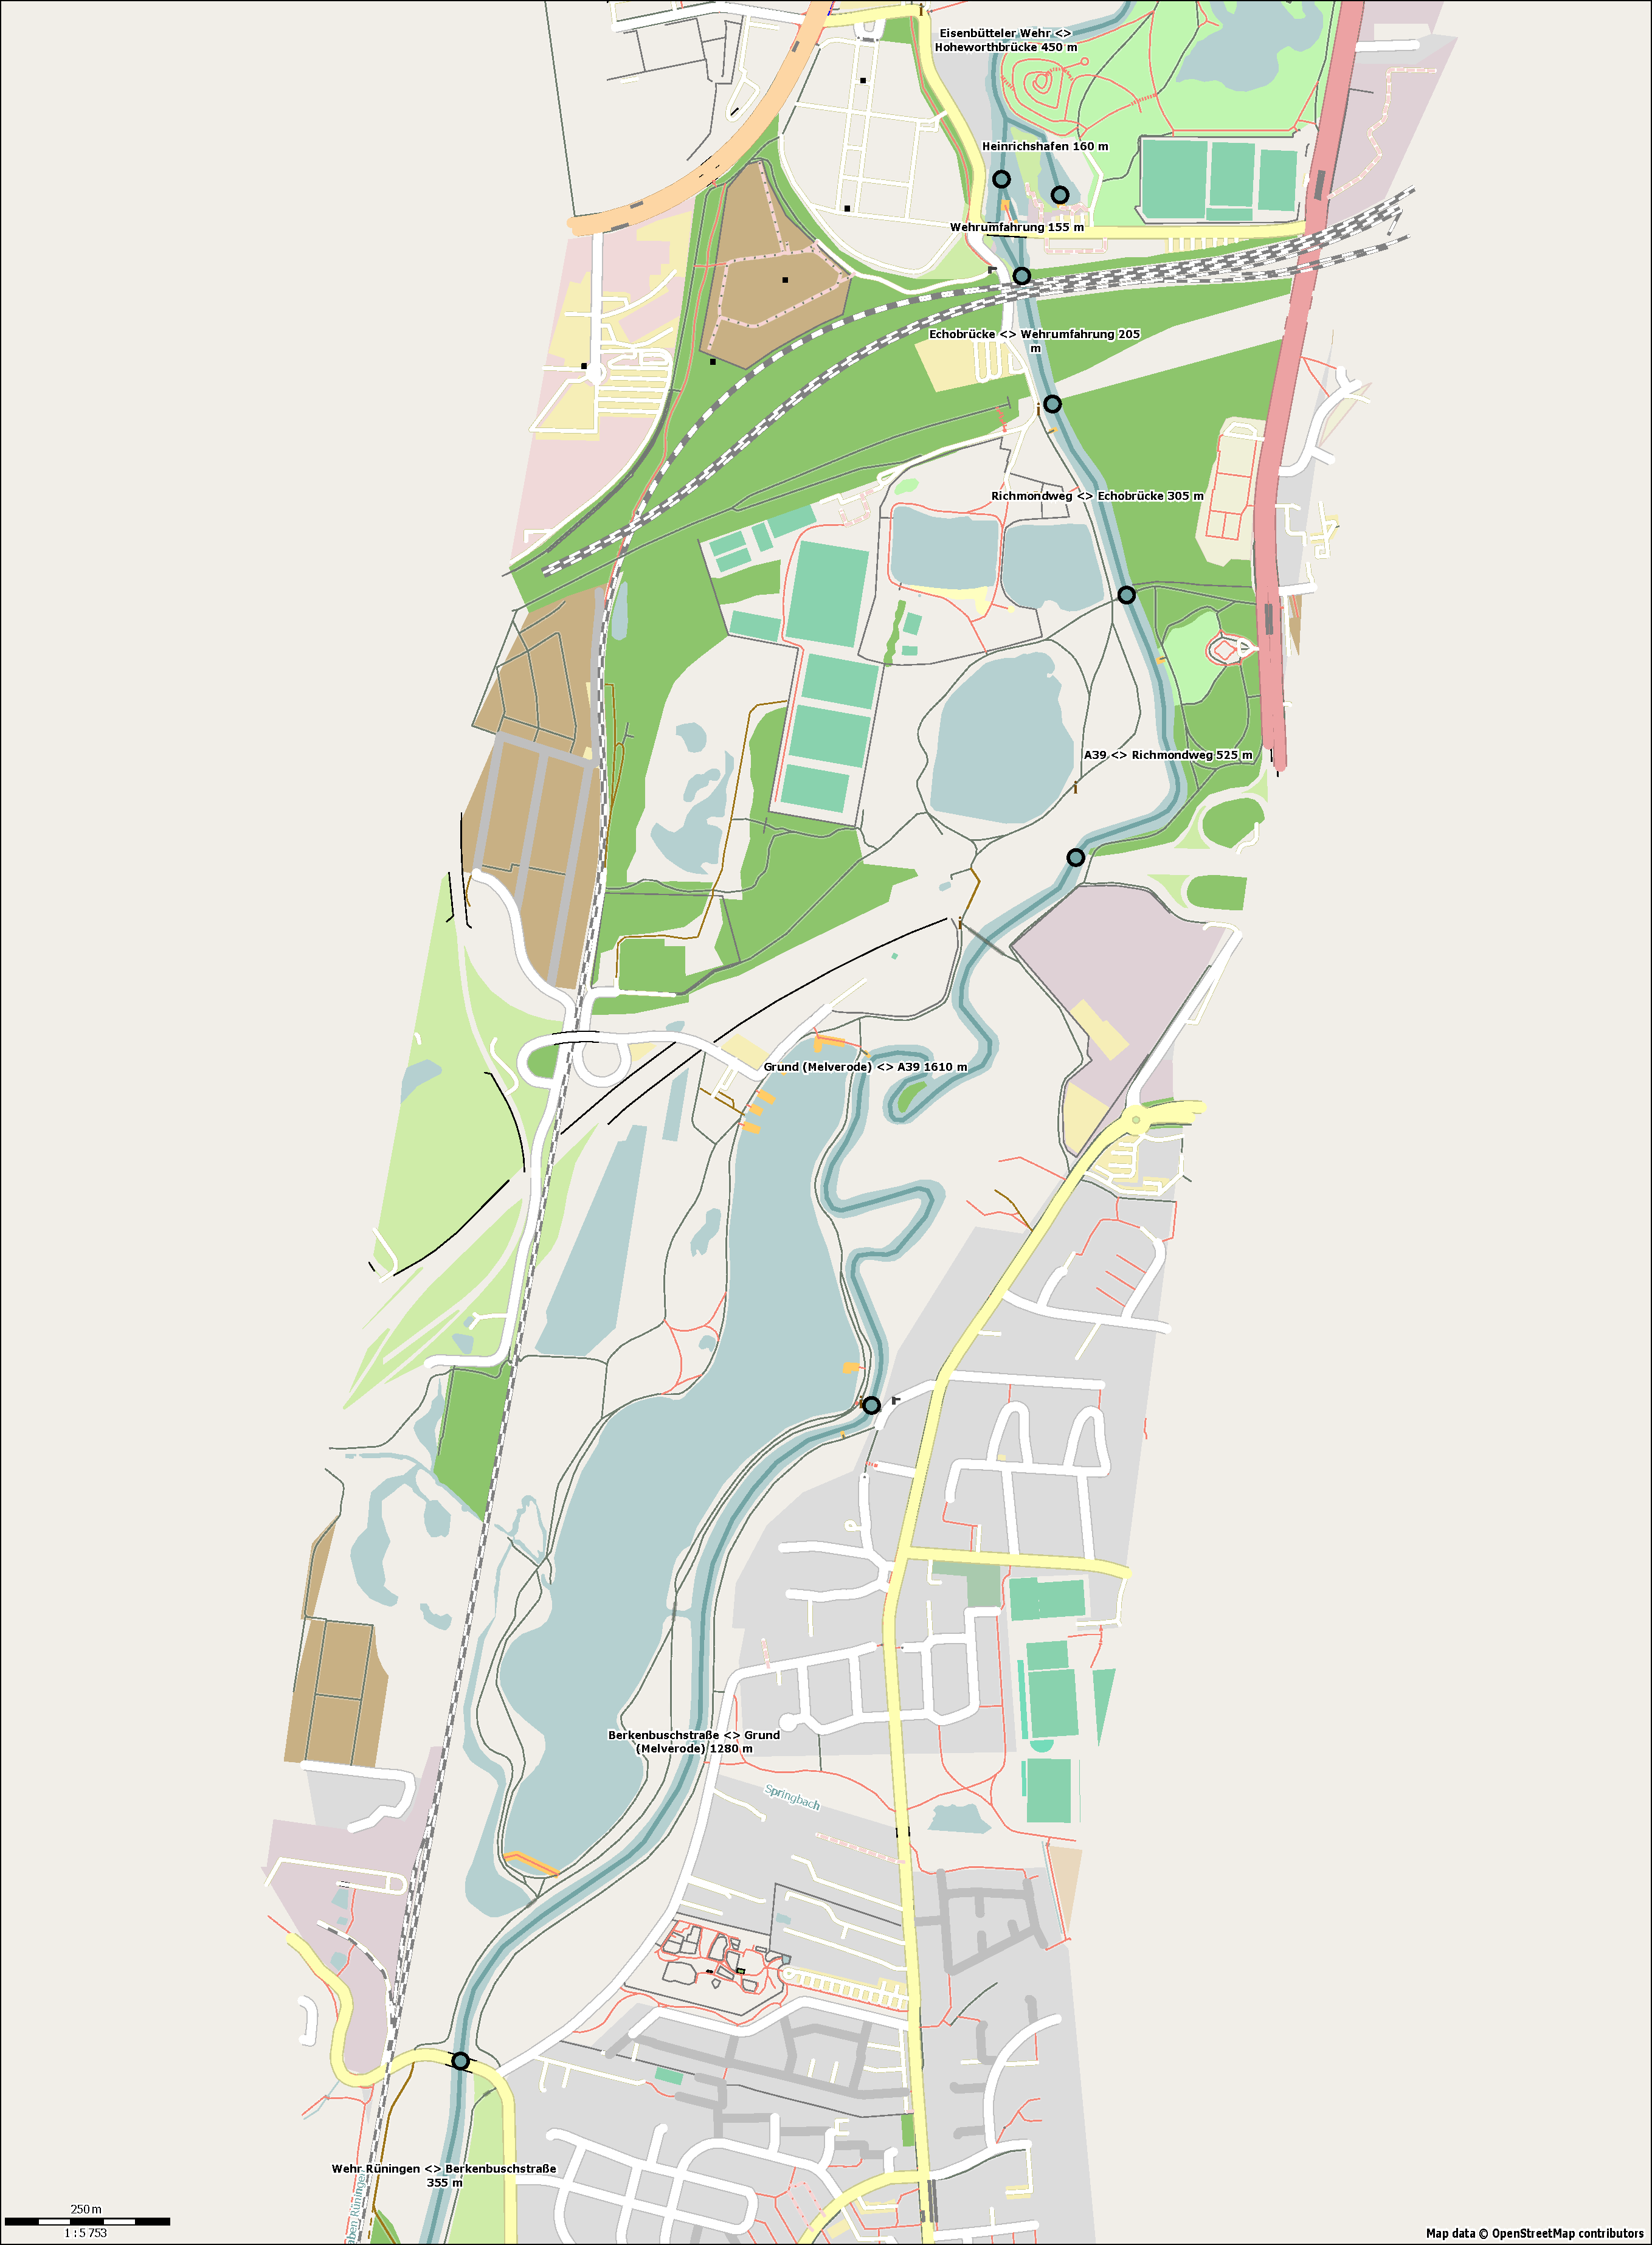
\includegraphics[max size={\textwidth}{0.95\textheight}]{../Result/BS_Sued2.pdf}
        \caption{Braunschweig-Melverode}
        \label{fig:map_BS2}
    \end{figure}
    \newpage
    
    \begin{figure}[!h]
        \centering
        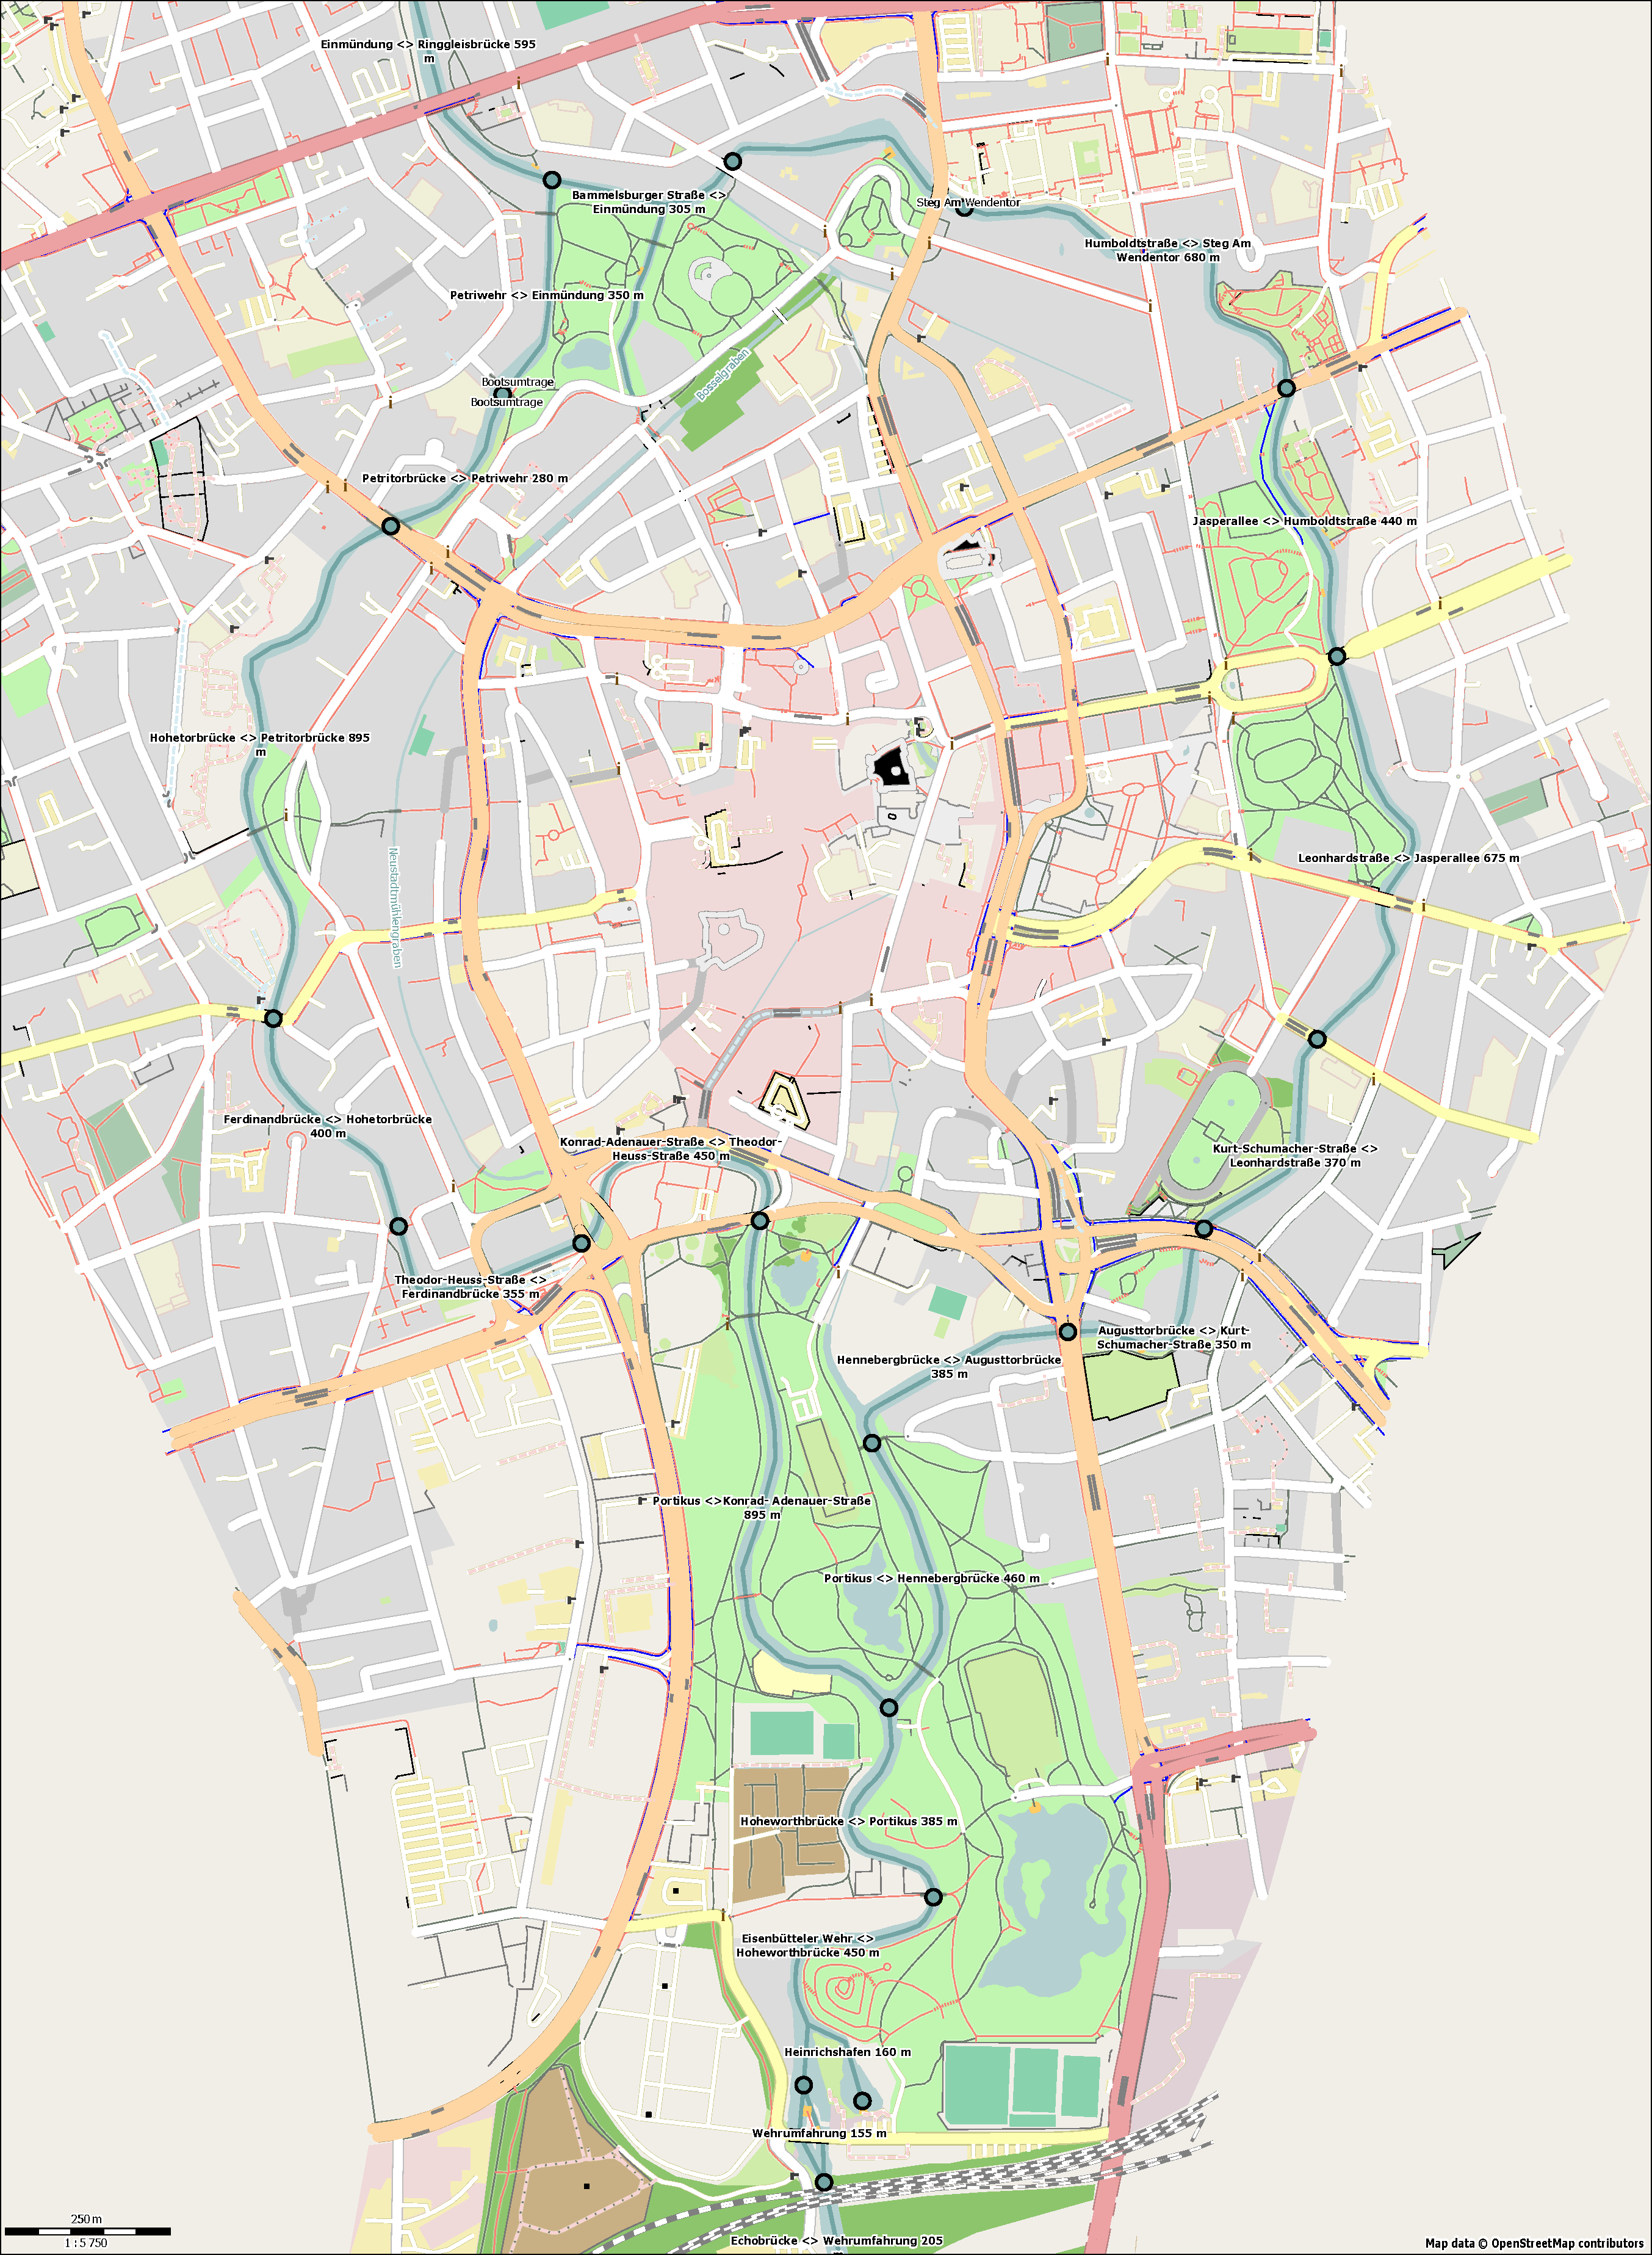
\includegraphics[max size={\textwidth}{0.95\textheight}]{../Result/BS_Okerumflut.pdf}
        \caption{Braunschweig-Innenstadt}
        \label{fig:map_BS3}
    \end{figure}
    \newpage
    
    \begin{figure}[!h]
        \centering
        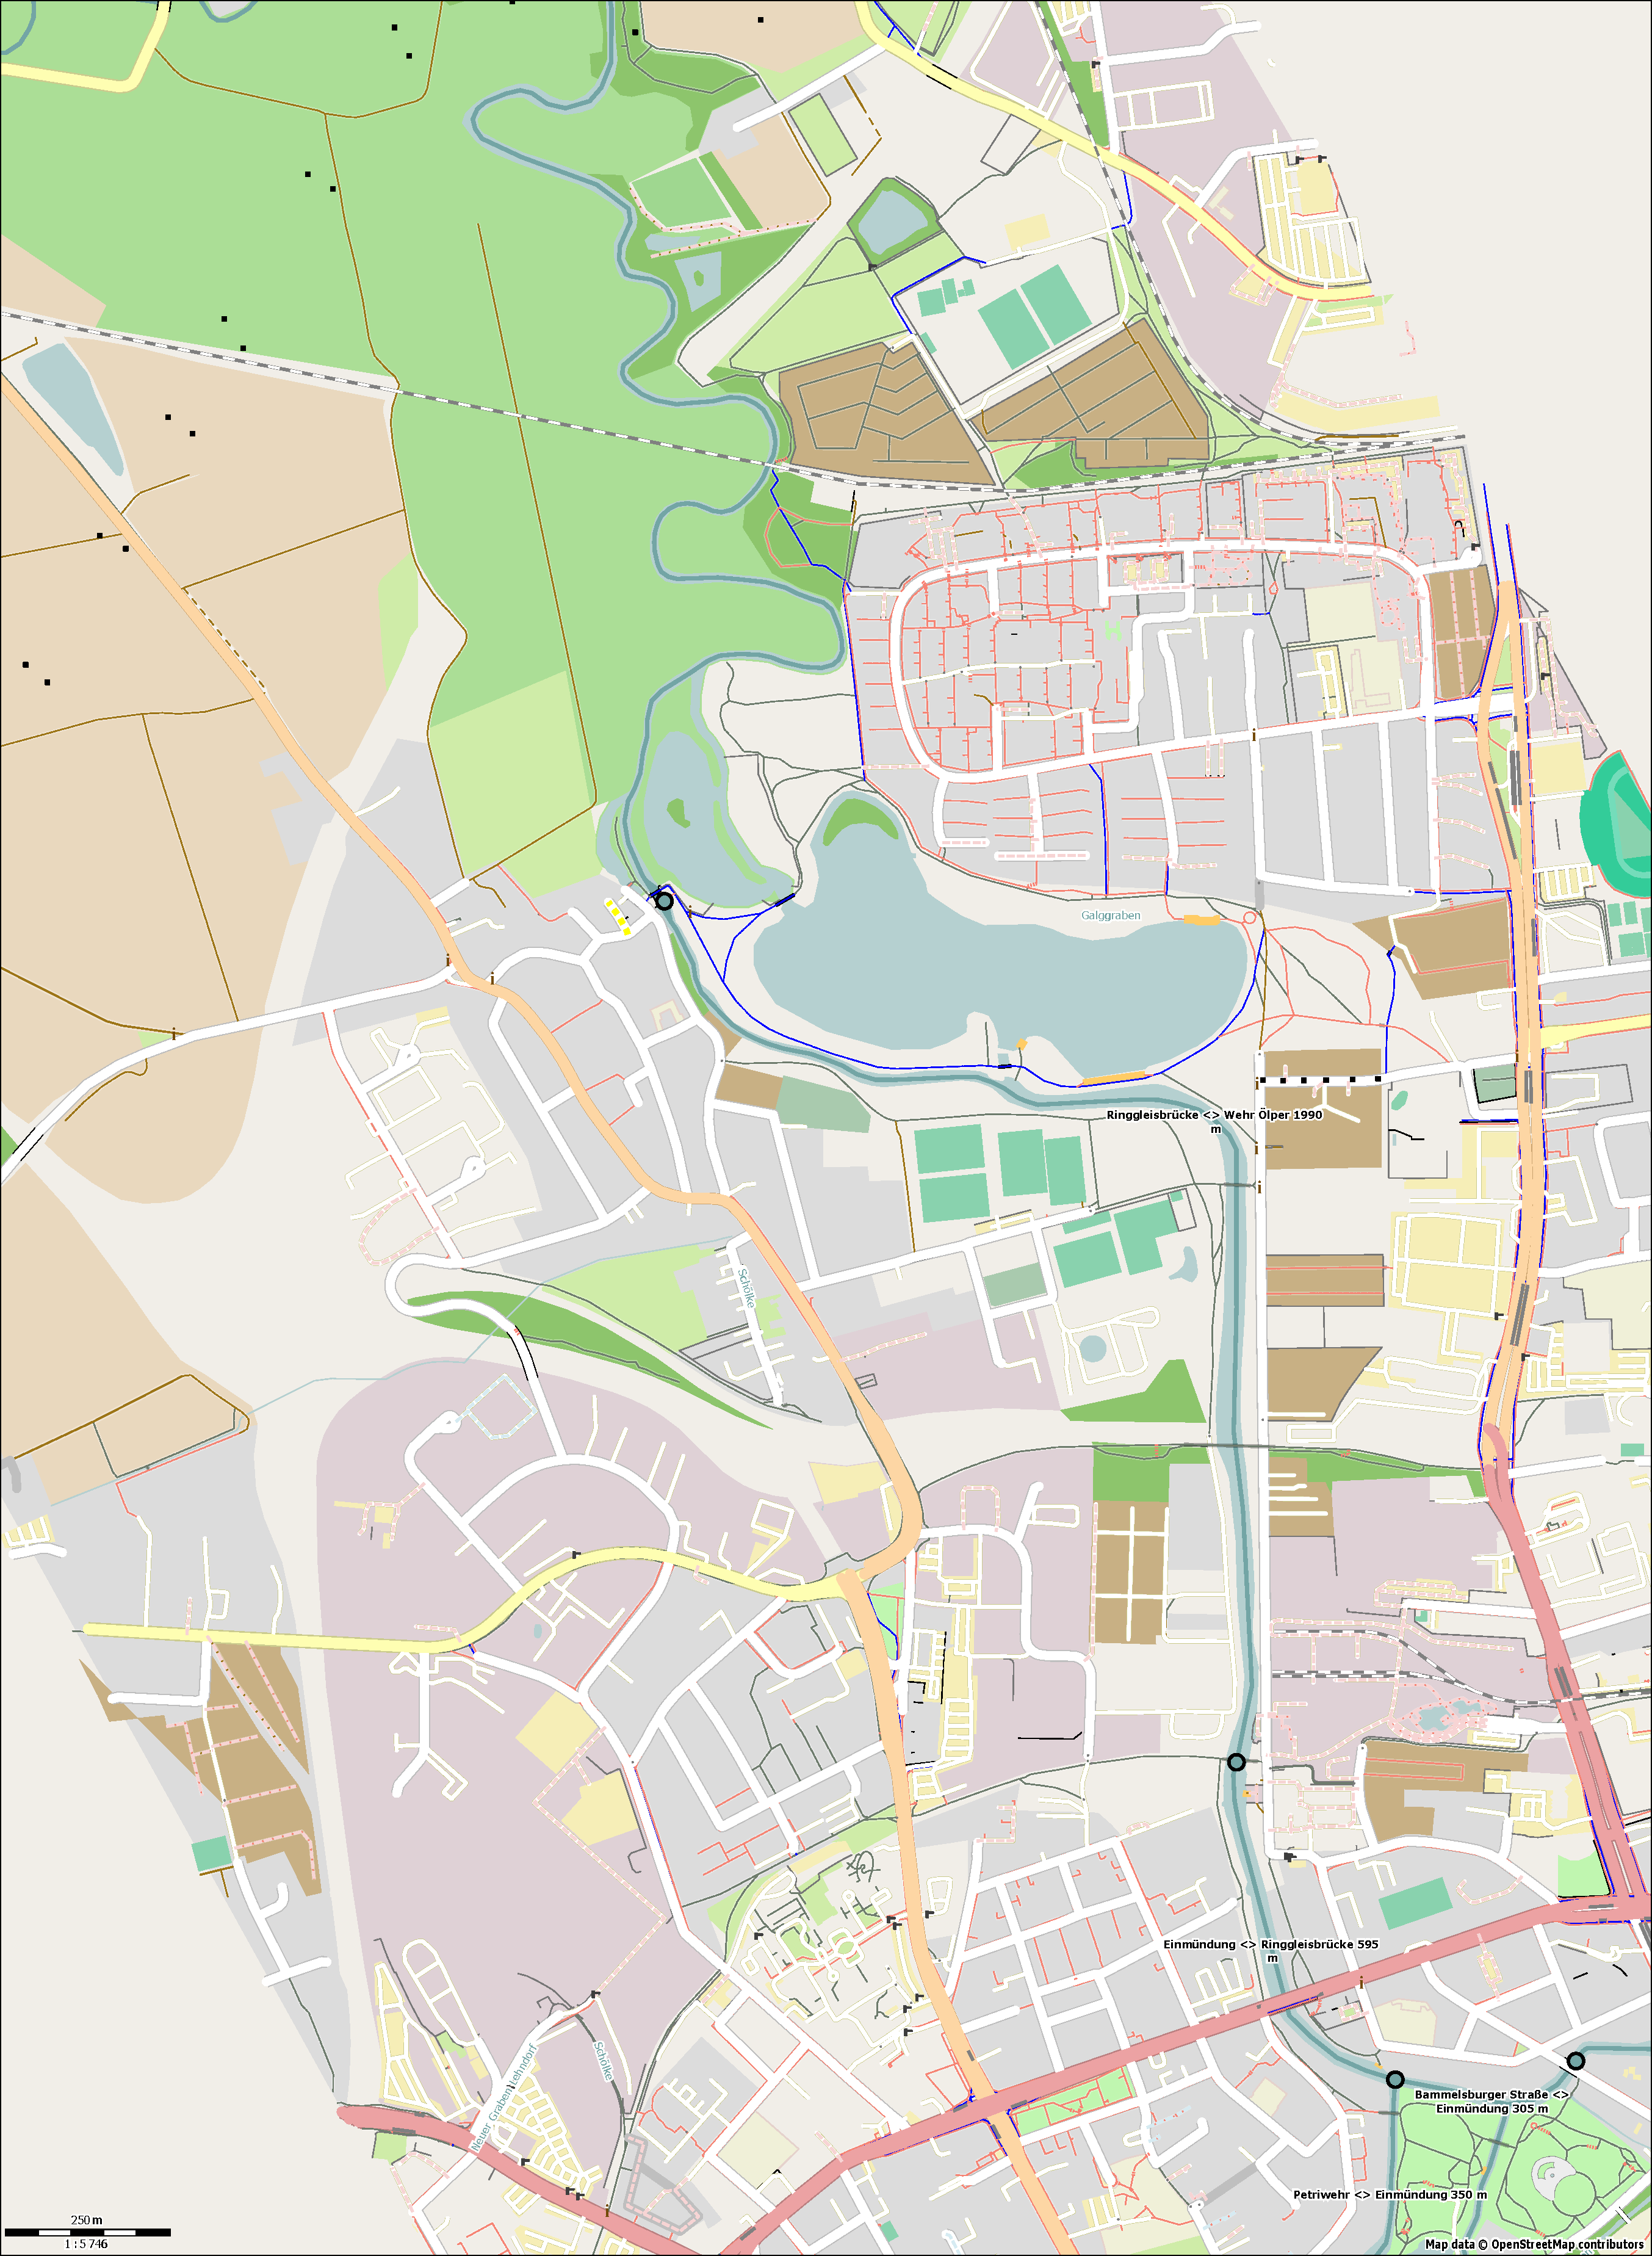
\includegraphics[max size={\textwidth}{0.95\textheight}]{../Result/BS_Nord.pdf}
        \caption{Braunschweig-Nordstadt}
        \label{fig:map_BS4}
    \end{figure}
    \newpage
    
%     \begin{figure}[!h]
%         \centering
%         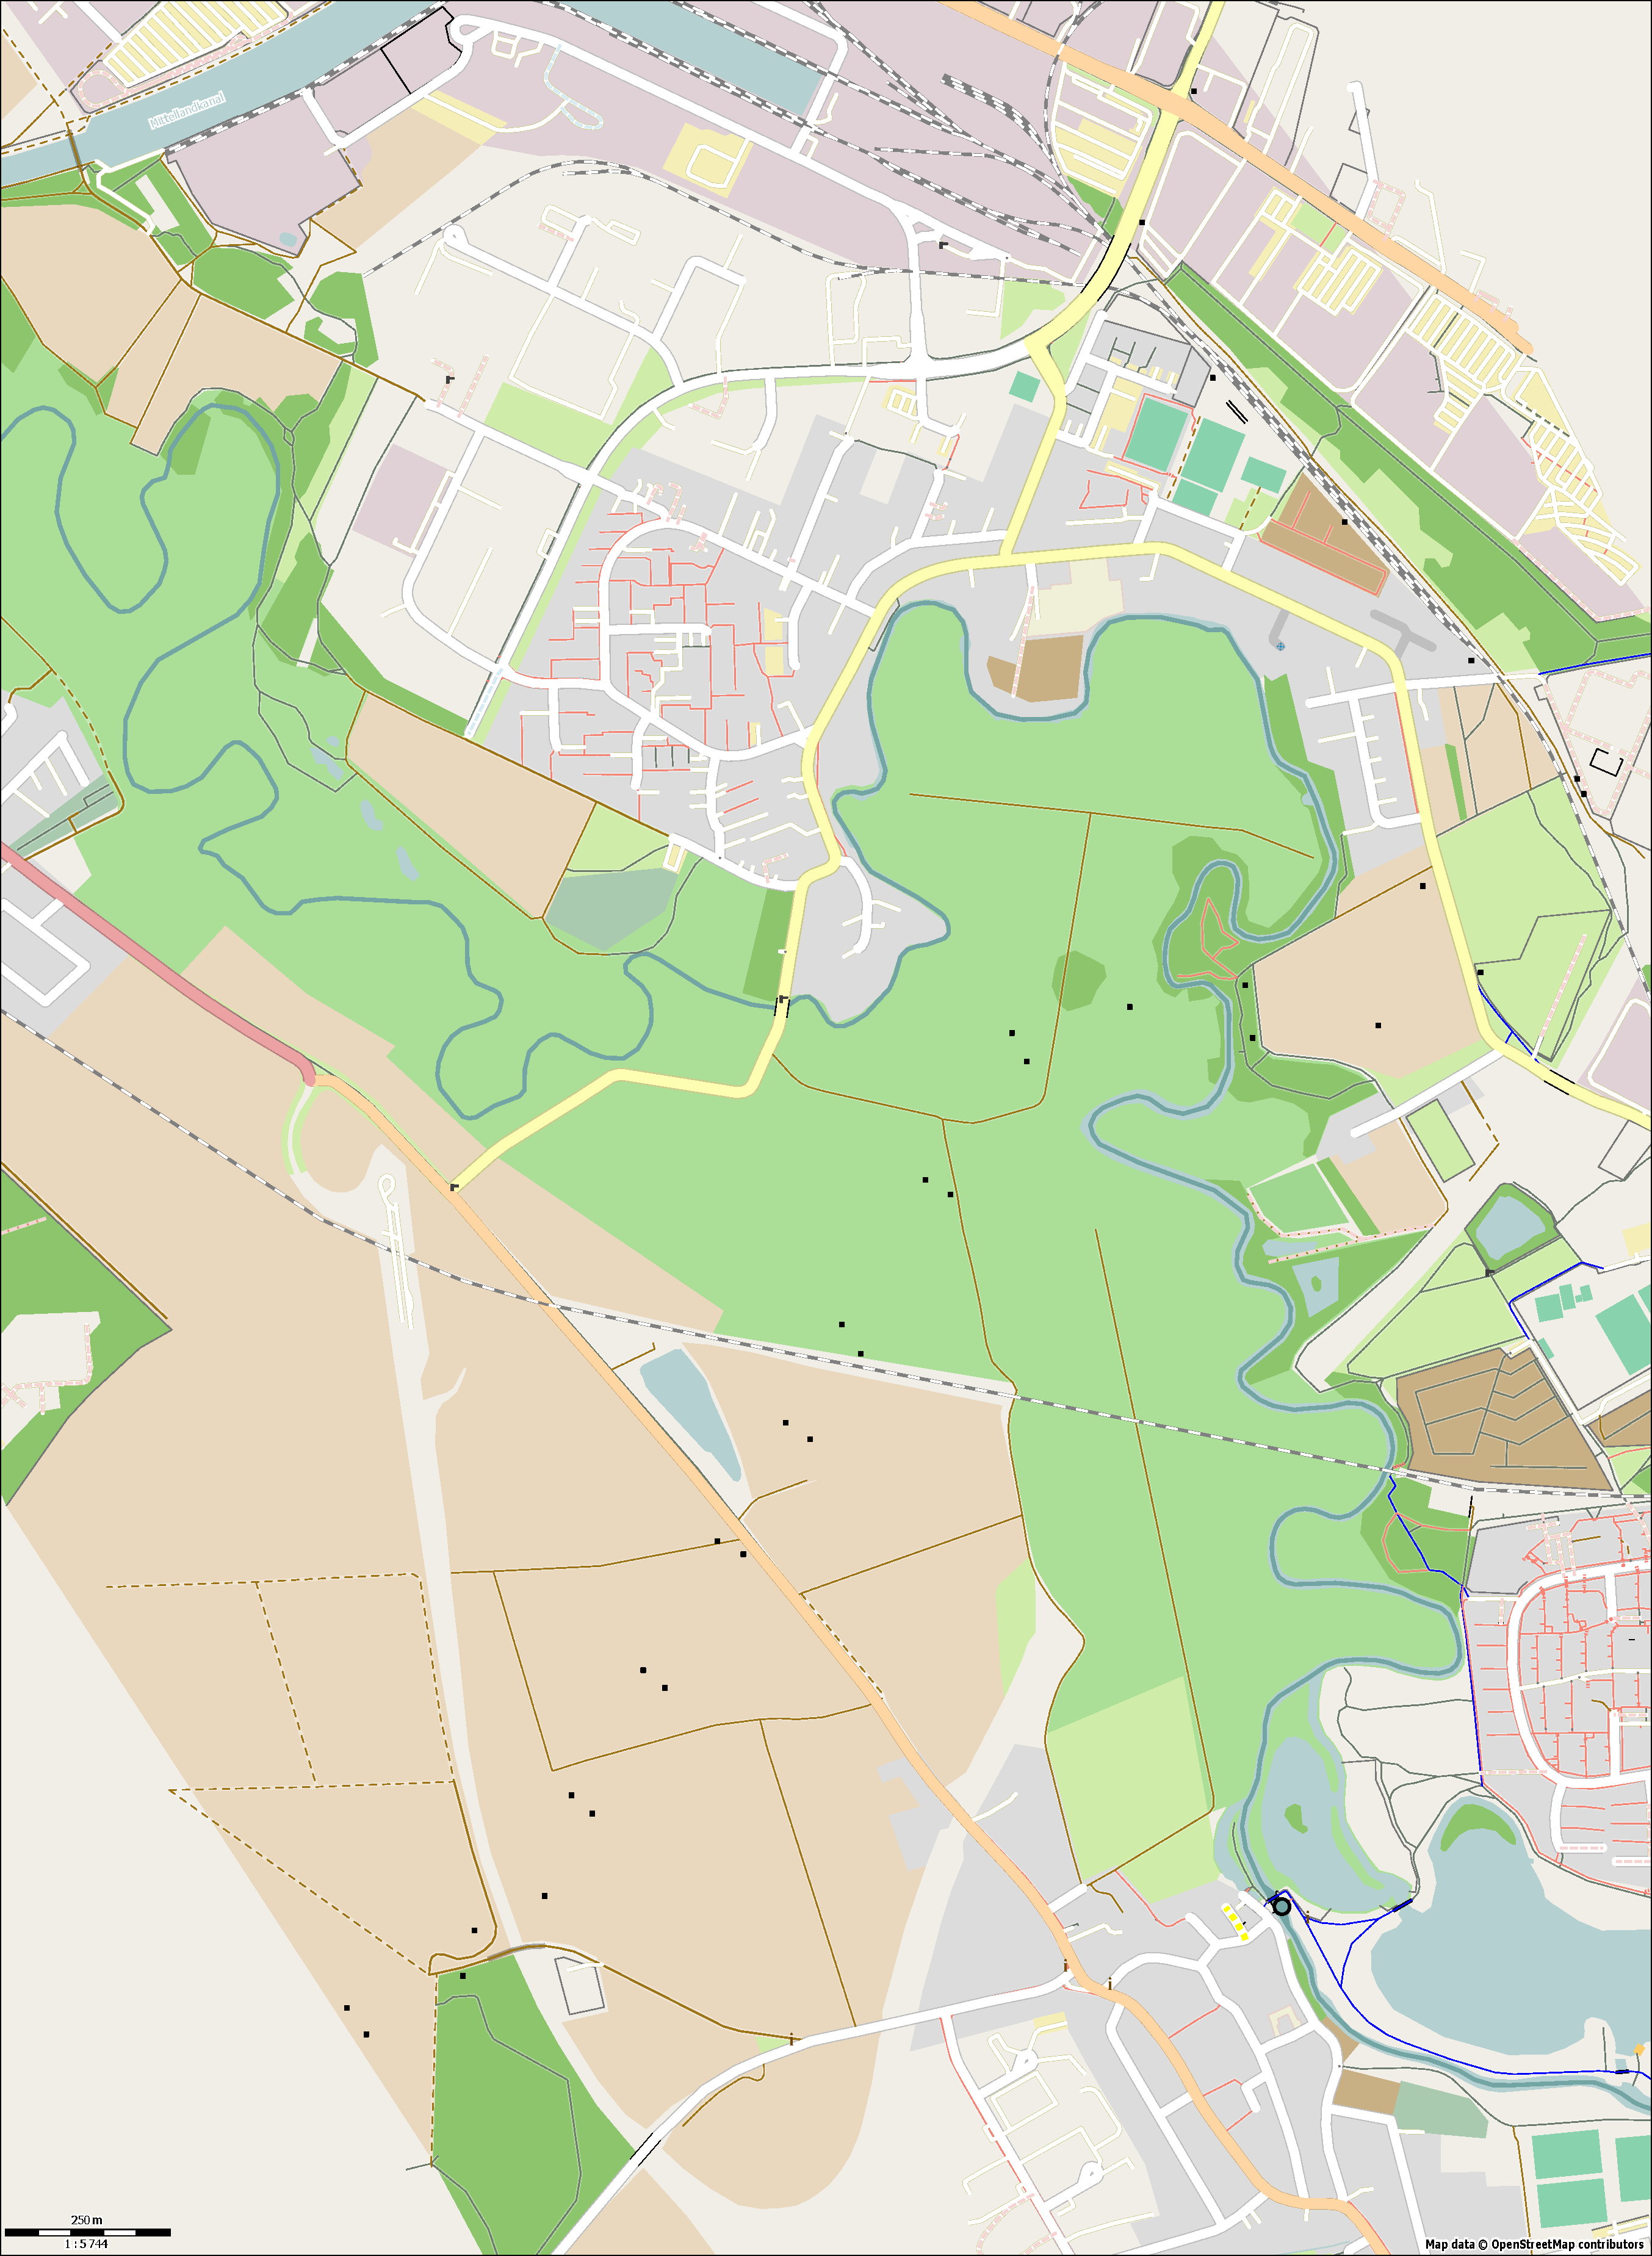
\includegraphics[max size={\textwidth}{0.95\textheight}]{../Result/BS_Nord2.pdf}
%         \caption{Braunschweig-Veltenhof}
%         \label{fig:map_BS5}
%     \end{figure}
%     \newpage
%     
%     \begin{figure}[!h]
%         \centering
%         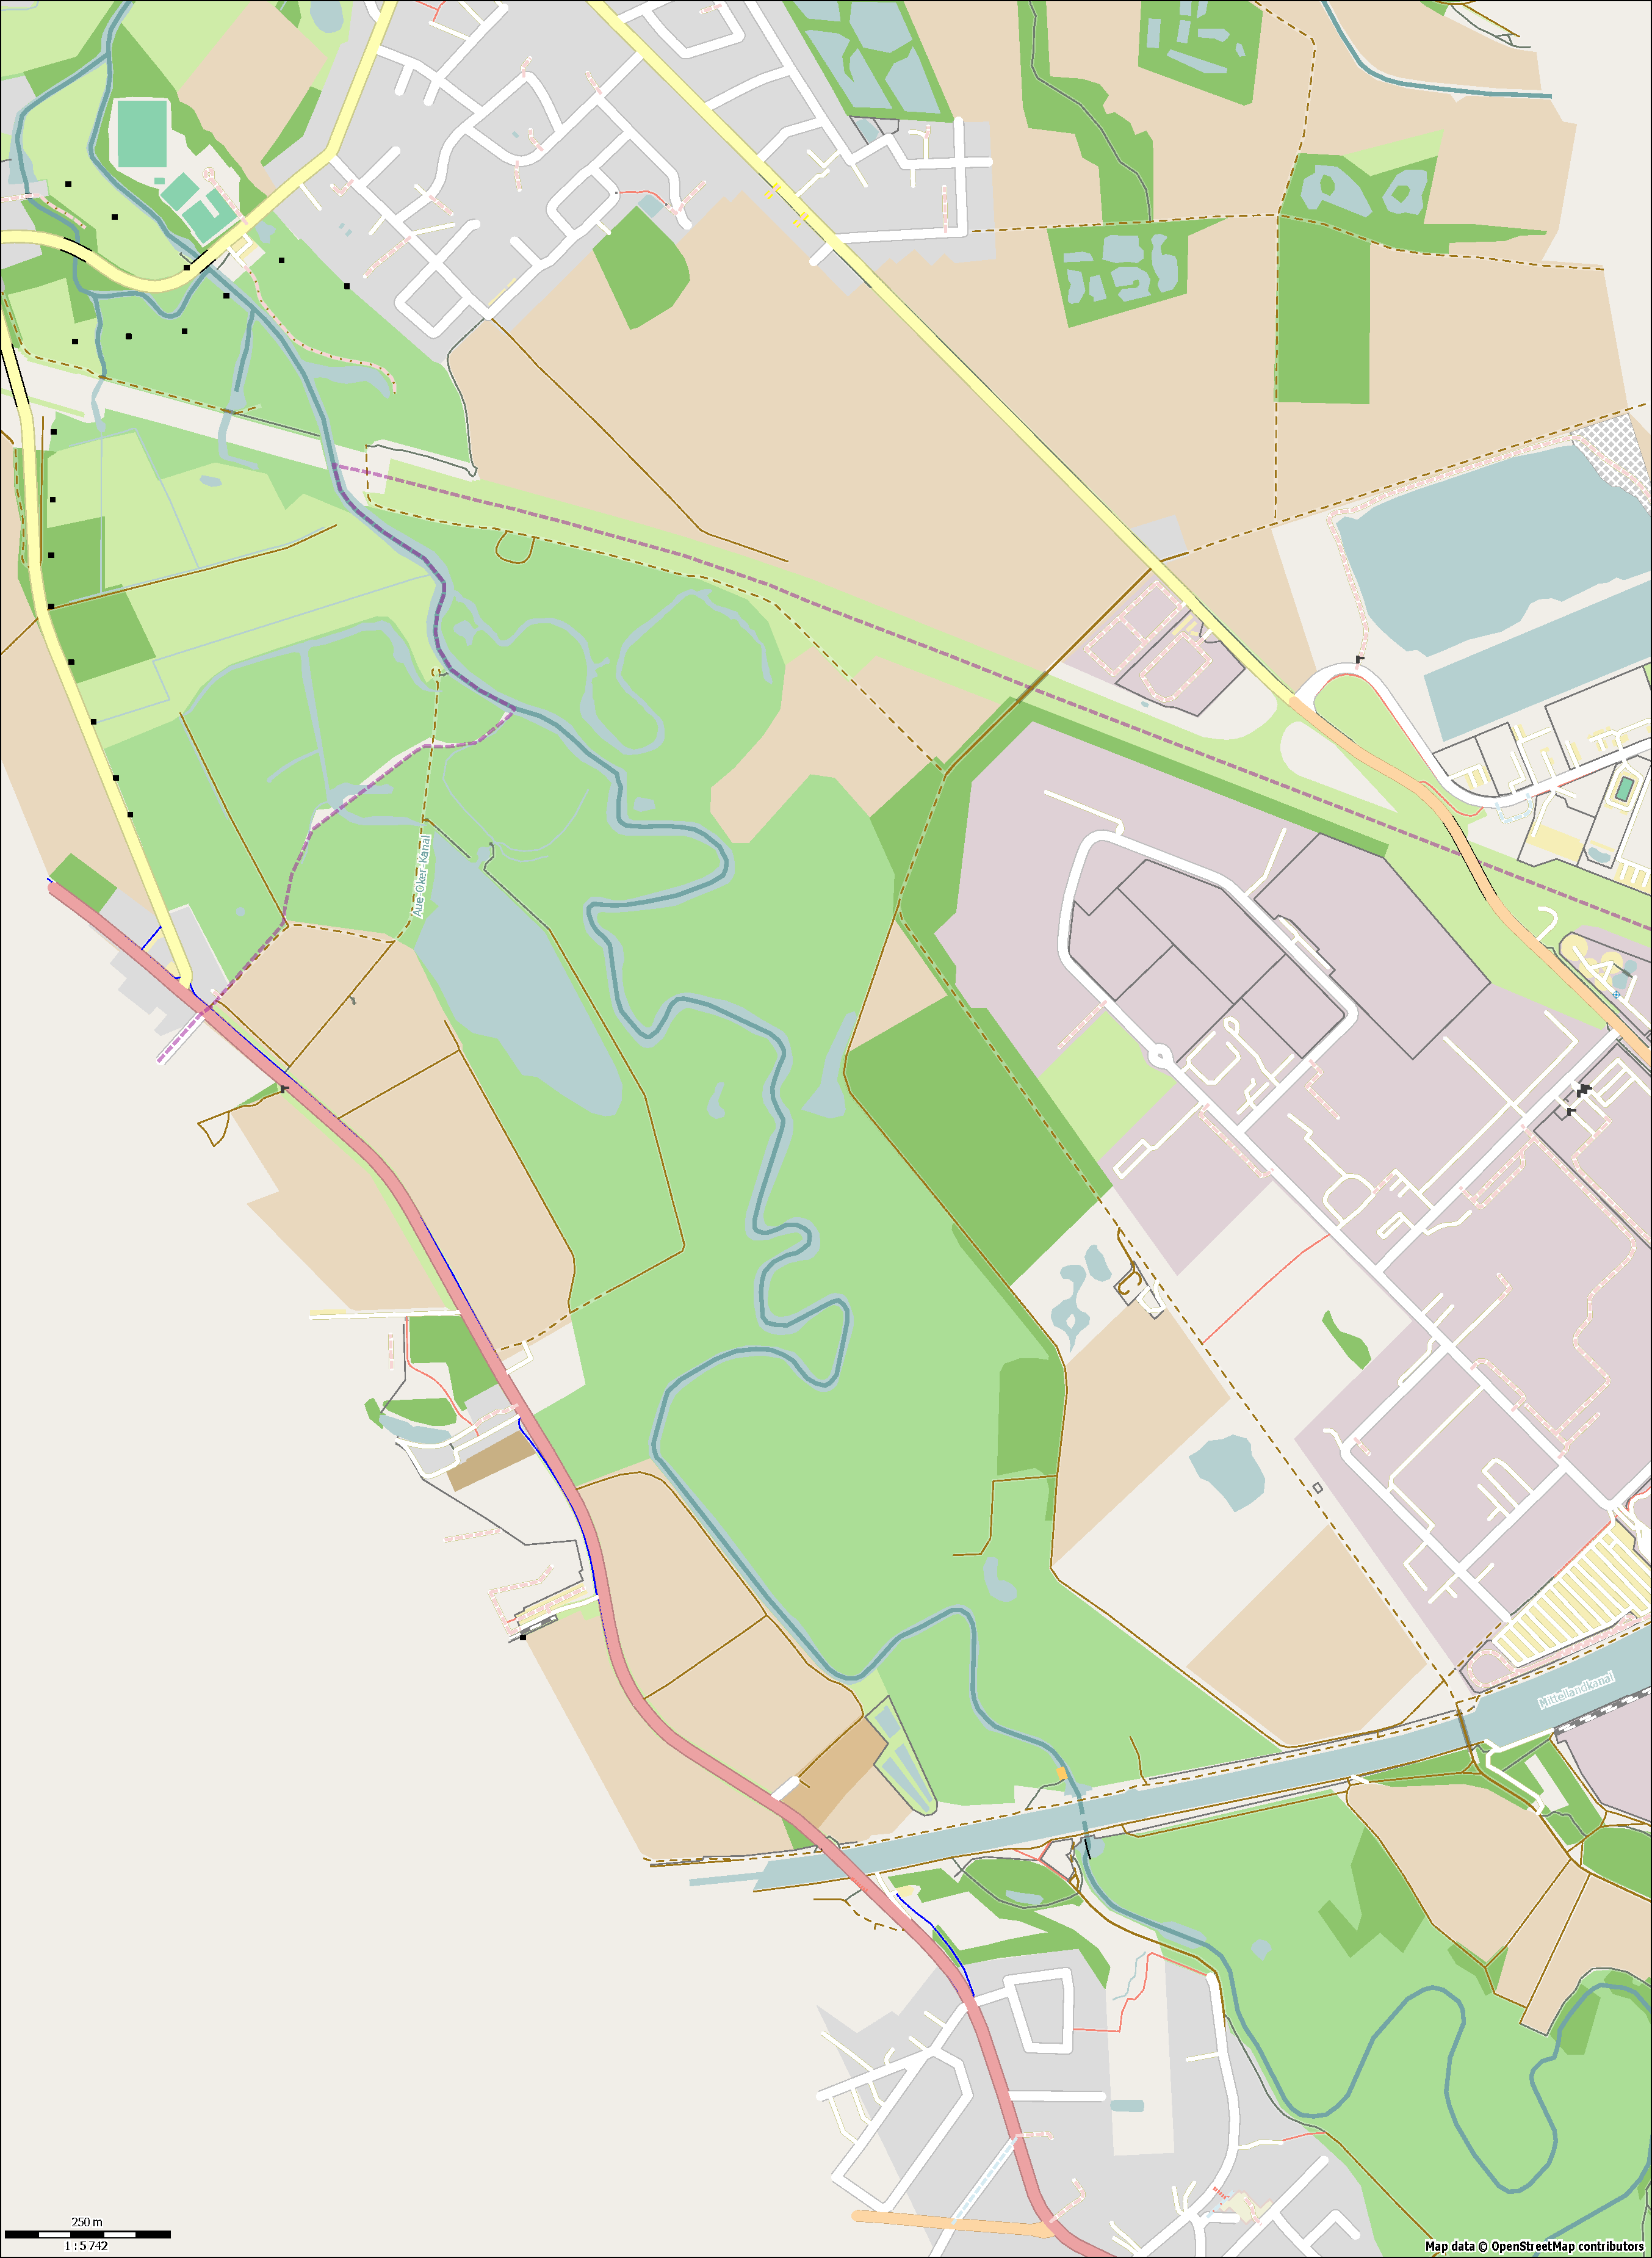
\includegraphics[max size={\textwidth}{0.95\textheight}]{../Result/GF.pdf}
%         \caption{Schwülper}  
%         \label{fig:map_GF}      
%     \end{figure}
\end{document}